% EMNLP 2023 style; pdfLaTeX recommended.
\pdfoutput=1
% Allow line breaks in long \url{...} (footnotes, etc.); must precede hyperref/url load.
\PassOptionsToPackage{hyphens}{url}

\documentclass[11pt]{article}

\usepackage[final]{EMNLP2023}

\usepackage{times}
\usepackage{latexsym}
\usepackage[T1]{fontenc}
\usepackage[utf8]{inputenc}
\usepackage{microtype}
\usepackage{graphicx}
\usepackage{booktabs}
\usepackage{tabularx}
\usepackage{array}
\usepackage{multirow}

% Figures: ship PDFs under report/figures/ for builds where ../results/ is absent (e.g.\ clean clone).
\graphicspath{{./figures/}{../results/figures/}}

\title{Dimension-Specific Reliability of LLM Judges:\\
  A Controlled Summarization Study with Human Gold}

\author{Abraham Paul Elenjical\thanks{Code and data: \url{https://github.com/abracodeabra1/emnlp-miniproject}.} \\
  Roll No.\ 2022114007 \\
  Evaluation Methods in NLP (2026)}

\begin{document}
\maketitle

\begin{abstract}
We study whether large language model (LLM) judges fail uniformly or \emph{dimension-specifically} on summarization, using a controlled setup: 50 CNN/Daily Mail articles, two comparable small instruct summarizers (Llama-3.2-1B-Instruct and Qwen2.5-1.5B-Instruct), and human ratings on four SummEval-style dimensions (coherence, consistency, fluency, relevance) from three annotators. Two API judges---\texttt{openai/gpt-oss-20b} and \texttt{qwen/qwen3-32b}---evaluate outputs under three protocols (direct scoring, pairwise comparison, and rubric-based structured scoring), with prompt wording, reference visibility, and presentation order varied. Consistency with the source lags coherence, fluency, and relevance in Spearman correlation with humans for both judges (e.g., GPT-OSS-20B reaches $\rho{=}0.64$ on consistency vs.\ $0.84$--$0.87$ on the other dimensions), supporting a dimension-specific reliability gap. Pairwise judgments agree with a human-derived preference in 82\% and 78\% of decidable cases yet show substantial order sensitivity (28\% strict reversals). Ten adversarial summaries (Gemini~2.5 Flash) further stress-test surface vs.\ factual behavior. The analysis goes beyond aggregate correlation: bias metrics, adversarial outcomes, and a rule-based failure taxonomy show where judges inflate scores, overlook inconsistencies, and conflate dimensions.
\end{abstract}

\section{Introduction}

LLM-as-a-judge is increasingly used to evaluate open-ended generation \citep{gu2024survey}. \citet{zheng2023judging} systematically study strong LLM judges and document biases including position, verbosity, and self-enhancement; separately, pairwise elicitation can be skewed by the order in which candidates appear \citep{wang2024largebench}. G-Eval shows that LLM-based scores track human judgments unevenly across tasks and are sensitive to chain-of-thought evaluation design \citep{liu2023geval}. For summarization, \citet{fabbri2021summeval} established human-validated multi-dimensional scores; subsequent work trains open evaluator LMs for direct and pairwise assessment with high human or proprietary-judge agreement \citep{kim2024prometheus2,zhu2024judgelm}. Separately, length-controlled variants of AlpacaEval formalize how auto-annotators can favor longer outputs and how to regress out that confound \citep{dubois2024length}.

This miniproject treats the LLM judge as an object of study: we ask when it aligns with a human gold standard, when it fails, and how sensitive conclusions are to prompts and presentation. Our central hypothesis is that correlation with humans will be higher on coherence and fluency than on \emph{consistency}, which requires checking facts against the source article rather than surface pattern matching.

\paragraph{Contributions.}
We present a controlled benchmark with two systems per article, a four-dimension human rubric with inter-annotator agreement, three judge protocols crossed with prompt and reference factors, meta-evaluation with correlation and bias analyses, ten adversarial probes, and a failure taxonomy. As an extension, we compare two hosted judge models (GPT-OSS-20B vs.\ Qwen3-32B) under identical prompts and data.

\section{Related Work}

\textbf{LLM judges and benchmarks.}
\citet{zheng2023judging} introduced MT-Bench and Chatbot Arena, popularizing pairwise LLM evaluation and documenting self-enhancement and other biases. \citet{wang2024largebench} document how presentation order skews pairwise LLM judgments. A recent survey synthesizes evaluation-of-evaluator methodology and bias taxonomies \citep{gu2024survey}.

\textbf{Summarization and rubrics.}
\citet{fabbri2021summeval} provide the SummEval corpus with human scores on coherence, consistency, fluency, and relevance---our annotation dimensions. \citet{liu2023geval} propose G-Eval, using chain-of-thought-style prompting for reference-free scoring on summarization and dialogue; we include a chain-of-thought-style prompt variant for comparison.

\textbf{Specialized judge models.}
Prometheus~2 \citep{kim2024prometheus2} and JudgeLM \citep{zhu2024judgelm} fine-tune open models as specialist judges. Our experiments use unrelated general chat endpoints on Groq with the same logical labels in code; we refer to them by their API model identifiers throughout.

\section{Task and Data}

\paragraph{Task.}
Open-domain \emph{single-document summarization}: given a news article, systems produce a short summary. We include challenging news-domain content and, separately, ten adversarial summaries (Section~\ref{sec:adversarial}).

\paragraph{Corpus.}
Articles come from the CNN/Daily Mail test split (version 3.0.0) distributed via Hugging Face Datasets \citep{hermann2015teaching}. Following SummEval's use of CNN/DM, we take the first 100 test articles as a pool, then draw a fixed 50-article subset (seed~42) so the study sits in the 40--60 example range required by the course. Each article is paired with two system summaries (100 scored items for item-level analyses).

\paragraph{Systems judged.}
Two small instruct models generate summaries in fp16: \textbf{Llama-3.2-1B-Instruct} and \textbf{Qwen2.5-1.5B-Instruct}. They are comparable in capacity and serve as the judged systems throughout.

\section{Human Evaluation}

\paragraph{Rubric.}
Three annotators rate each summary on four dimensions on a 1--5 Likert scale, with definitions aligned to SummEval: coherence (structure), consistency (factual alignment with the article), fluency (grammar and naturalness), and relevance (coverage of important content) \citep{fabbri2021summeval}.

\paragraph{Procedure.}
Annotators use a lightweight web interface to rate summaries incrementally; per-annotator files are merged and aggregated to per-item mean scores, which define the gold standard used for judge evaluation.

\paragraph{Agreement.}
Table~\ref{tab:iaa} reports Krippendorff's $\alpha$ and the mean pairwise Cohen's $\kappa$ across annotator pairs. Agreement is strong on coherence, fluency, and relevance, but clearly lower on consistency---the dimension that most directly encodes source faithfulness---mirroring the difficulty we later observe for automatic judges.

\begin{table}[t]
\centering
\footnotesize
\setlength{\tabcolsep}{3pt}
\begin{tabular}{@{}lcccc@{}}
\toprule
 & Coh. & Con. & Flu. & Rel. \\
\midrule
Kripp.\ $\alpha$ & 0.878 & 0.615 & 0.893 & 0.888 \\
Mean $\kappa$ & 0.882 & 0.642 & 0.888 & 0.886 \\
\bottomrule
\end{tabular}
\caption{Inter-annotator agreement on the study subset ($n{=}50$ articles, three annotators). Kripp.\ $=$ Krippendorff; $\kappa$ $=$ Cohen's $\kappa$ (mean pairwise).}
\label{tab:iaa}
\end{table}

Human consistency agreement (Krippendorff $\alpha{=}0.62$) is the weakest of the four dimensions, reflecting how hard source-grounded judgments are even for humans. We therefore expect automatic judges to struggle most on the same dimension when aligned to this gold.

\section{LLM Judges and Experimental Factors}
\label{sec:judges}

\paragraph{Judge models (extension: two judges).}
All judge calls use hosted APIs. We report two Groq chat models: \texttt{openai/gpt-oss-20b} (``GPT-OSS-20B'') and \texttt{qwen/qwen3-32b} (``Qwen3-32B''). They are evaluated under identical prompts and data splits.

\paragraph{Three evaluation modes.}
\textbf{(A) Direct scoring:} one dimension at a time, integer 1--5. \textbf{(B) Pairwise:} which summary is better overall; we elicit both A$\rightarrow$B and B$\rightarrow$A orderings to study position effects \citep{wang2024largebench,zheng2023judging}. \textbf{(C) Rubric-based:} all four dimensions scored in one call with explicit per-dimension criteria. Each mode is run across prompt variants and reference conditions (below).

\section{Prompt and Reference Sensitivity}

We vary \textbf{prompt wording} across three variants: \emph{minimal} (short instruction), \emph{standard} (brief rubric text per dimension where applicable), and \emph{cot} (criteria plus step-by-step reasoning before the score), following the spirit of G-Eval \citep{liu2023geval}. We vary \textbf{reference visibility}: reference highlights may be included for calibration or omitted. Pairwise mode uses the same variant grid plus order reversal.

\section{Meta-Evaluation and Bias Analysis}
\label{sec:meta}

\paragraph{Alignment with humans.}
Table~\ref{tab:corr} reports Spearman $\rho$ between judge scores and human means ($n{=}100$ summary-level items per dimension), using the \emph{standard} prompt without reference. Table~\ref{tab:kendall} gives Kendall $\tau$ for the same items; rank agreement follows the same pattern as $\rho$. Figure~\ref{fig:corr} plots $\rho$ by dimension: both judges track humans best on relevance, while consistency is the weakest link, especially for Qwen3-32B ($\rho{=}0.57$).

\begin{table}[t]
\centering
\small
\begin{tabular}{lcccc}
\toprule
Judge & Coh. & Con. & Flu. & Rel. \\
\midrule
GPT-OSS-20B & 0.839 & 0.638 & 0.810 & 0.868 \\
Qwen3-32B & 0.678 & 0.569 & 0.740 & 0.862 \\
\bottomrule
\end{tabular}
\caption{Spearman $\rho$ vs.\ human gold (standard prompt, no reference). All $p{<}0.001$.}
\label{tab:corr}
\end{table}

\begin{table}[t]
\centering
\small
\begin{tabular}{lcccc}
\toprule
Judge & Coh. & Con. & Flu. & Rel. \\
\midrule
GPT-OSS-20B & 0.735 & 0.523 & 0.702 & 0.755 \\
Qwen3-32B & 0.579 & 0.475 & 0.641 & 0.746 \\
\bottomrule
\end{tabular}
\caption{Kendall $\tau$ vs.\ human gold (same setting as Table~\ref{tab:corr}).}
\label{tab:kendall}
\end{table}

\begin{figure}[t]
\centering
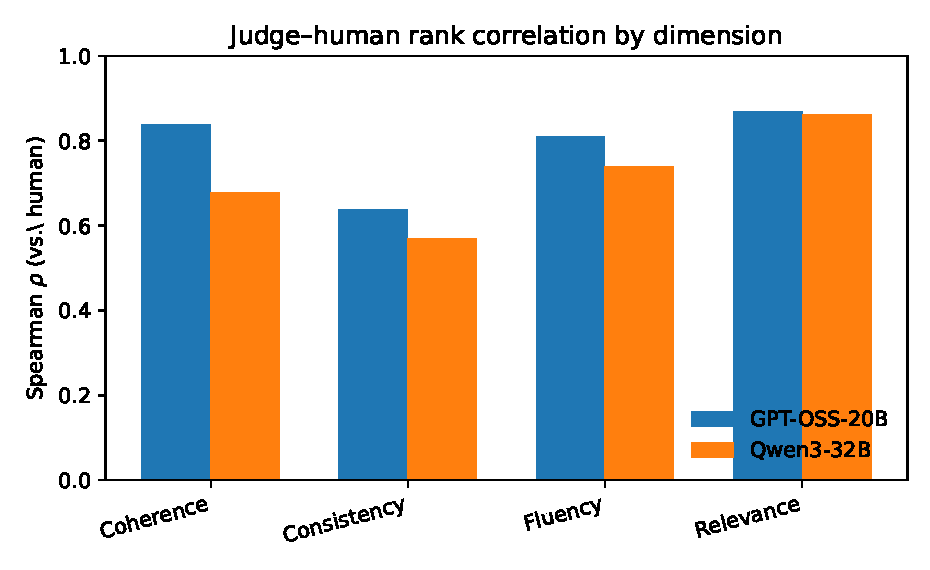
\includegraphics[width=\columnwidth]{corr_by_dimension_two_judges.pdf}
\caption{Spearman $\rho$ by dimension for the two judges (same setting as Table~\ref{tab:corr}).}
\label{fig:corr}
\end{figure}

\subsection{Mean absolute error and systematic bias}
Correlation alone can mask calibration: a judge may preserve ranks while systematically shifting levels. Table~\ref{tab:mae} reports mean absolute error (MAE) between judge and human scores and the mean signed error (positive $=$ judge higher than humans). GPT-OSS-20B is closest on fluency (MAE 0.57) but still tends to \emph{inflate} coherence and consistency relative to annotators (mean biases ${+}0.81$ and ${+}0.27$). Qwen3-32B shows much larger MAE on coherence, consistency, and fluency (${\sim}1.3$--1.8 points on the 1--5 scale) with strong positive bias on those three dimensions, while staying closer on relevance. Together with Table~\ref{tab:corr}, this suggests Qwen3-32B is not only less rank-aligned but also systematically lenient on surface-oriented dimensions.

\begin{table}[t]
\centering
\footnotesize
\begin{tabular}{@{}llcc@{}}
\toprule
Judge & Dim. & MAE & Mean bias \\
\midrule
\multirow{4}{*}{GPT-OSS-20B} & Coh. & 0.87 & $+0.81$ \\
 & Con. & 0.79 & $+0.27$ \\
 & Flu. & 0.57 & $+0.31$ \\
 & Rel. & 0.70 & $-0.63$ \\
\midrule
\multirow{4}{*}{Qwen3-32B} & Coh. & 1.79 & $+1.79$ \\
 & Con. & 1.59 & $+1.57$ \\
 & Flu. & 1.31 & $+1.31$ \\
 & Rel. & 0.53 & $-0.32$ \\
\bottomrule
\end{tabular}
\caption{Calibration vs.\ human gold (direct scores, standard, no reference; $n{=}100$ per cell). Mean bias $=$ mean(judge $-$ human).}
\label{tab:mae}
\end{table}

\subsection{Rubric mode vs.\ humans and vs.\ direct scoring}
Rubric-based calls score all four dimensions in one generation step. Table~\ref{tab:rubric} shows Spearman $\rho$ between rubric outputs and human means under the same no-reference, \emph{standard} prompt setting. GPT-OSS-20B loses only modestly relative to direct scoring (e.g., coherence 0.80 vs.\ 0.84); Qwen3-32B degrades more on coherence and consistency but remains strong on relevance (0.81). For both judges, rubric and direct scores on the same summary--dimension are highly rank-correlated (Spearman $\rho$ between 0.80 and 0.93), so the two elicitation styles largely agree with each other even when they drift from humans.

\begin{table}[t]
\centering
\footnotesize
\begin{tabular}{@{}lcccc@{}}
\toprule
Judge & Coh. & Con. & Flu. & Rel. \\
\midrule
GPT-OSS-20B & 0.798 & 0.616 & 0.721 & 0.797 \\
Qwen3-32B & 0.543 & 0.494 & 0.544 & 0.806 \\
\bottomrule
\end{tabular}
\caption{Rubric-mode Spearman $\rho$ vs.\ human gold (standard, no reference).}
\label{tab:rubric}
\end{table}

\subsection{Inter-judge agreement}
We also measure agreement \emph{between} the two judges by correlating their direct scores on identical summary--dimension pairs. Spearman $\rho$ is 0.76 on relevance, 0.65 on fluency, 0.57 on coherence, but only 0.31 on consistency (all $p{<}0.001$). Judges therefore disagree most on the same dimension where each is least aligned with humans, which complicates using a single API judge as a stand-in for community judgment.

\subsection{Sensitivity of consistency correlation to prompt wording}
Table~\ref{tab:promptcons} fixes the dimension to consistency and varies only the prompt family (minimal, standard, cot), still without reference. GPT-OSS-20B's $\rho$ swings from 0.76 (minimal) down to 0.64 (standard) and back to 0.76 (cot); Qwen3-32B moves between 0.57 and 0.67. A single ``best'' prompt is not obvious, but the spread shows that measured human alignment for faithfulness is not stable under modest instruction changes.

\begin{table}[t]
\centering
\footnotesize
\begin{tabular}{@{}lccc@{}}
\toprule
Judge & Min. & Std. & CoT \\
\midrule
GPT-OSS-20B & 0.759 & 0.638 & 0.763 \\
Qwen3-32B & 0.674 & 0.569 & 0.630 \\
\bottomrule
\end{tabular}
\caption{Spearman $\rho$ (consistency dimension only) vs.\ human gold across prompt variants, no reference.}
\label{tab:promptcons}
\end{table}

\paragraph{Pairwise agreement with humans.}
For each article we define a human preference by comparing the mean of the four human dimension scores for summary~A vs.\ summary~B. On 49 articles with a strict preference (one tie on mean scores), GPT-OSS-20B's pairwise winner under the standard no-reference A$\rightarrow$B setting matches the human preference in 40 cases (81.6\%); Qwen3-32B in 38 (77.6\%). Thus head-to-head agreement is respectable but not sufficient for unattended use.

\paragraph{Pairwise protocol stability.}
For both judges, only 72\% of articles yield the same \emph{model-level} winner under both presentation orders (first-slot win rates 0.58 and 0.56, position-bias scores 0.16 and 0.12). Independently, a strict reversal check flags 28\% of articles (14/50) where the declared winner letter stays the same across orders even though the better \emph{model} should flip---a symptom of position-dependent behavior.

\paragraph{Verbosity, reference, and prompt sensitivity.}
Spearman correlations between scores and summary length are small and not significant for either judge on most dimensions (absolute $r$ below 0.15), so we do not find a strong linear verbosity confound in this sample. Including the reference summary slightly \emph{improves} consistency correlation for both judges ($\Delta\rho{=}{+}0.04$ for GPT-OSS-20B; ${+}0.01$ for Qwen3-32B) while modestly lowering several other correlations for Qwen3-32B, suggesting reference text can redistribute judge attention across dimensions. Prompt sensitivity, measured as the standard deviation of $\rho$ across minimal/standard/cot without reference, is largest for \emph{consistency} (0.058 GPT-OSS-20B; 0.043 Qwen3-32B), indicating that how one asks for faithfulness shifts measured alignment more than for surface dimensions.

\paragraph{Head-to-head system preference.}
In pairwise AB runs (standard, no reference), the Llama-generated summary is chosen 57\% (GPT-OSS-20B) and 60\% (Qwen3-32B) of the time. These are not ``self-preference'' effects for the judges (different model families); they indicate a systematic tilt toward one system under pairwise elicitation, which should be interpreted alongside direct-score correlations.

\begin{table}[t]
\centering
\footnotesize
\begin{tabularx}{\columnwidth}{@{}>{\raggedright\arraybackslash}p{0.28\columnwidth} X@{}}
\toprule
Bias / stability & Operationalization and headline result \\
\midrule
Position & First-slot win rate above 0.5 and 28\% order-linked reversal rate (Section~\ref{sec:meta}). \\
Verbosity & Spearman $r$ between score and word count: near null across dimensions. \\
Reference & $\Delta\rho$ on consistency positive with reference for both judges. \\
Prompt & Largest std.\ of $\rho$ across wording variants on consistency ($>$0.04). \\
\bottomrule
\end{tabularx}
\caption{Bias and sensitivity analyses (see Section~\ref{sec:meta} for numeric detail).}
\label{tab:bias}
\end{table}

\section{Adversarial Evaluation}
\label{sec:adversarial}

We construct ten adversarial summaries with \textbf{Gemini~2.5 Flash}, starting from fluent Llama-generated references: four \emph{fluent inconsistent} rewrites (subtle factual errors), three \emph{correct but poorly written} rewrites, and three \emph{meaning-shift} paraphrases. Table~\ref{tab:advdir} summarizes mean \emph{consistency} scores on the good vs.\ adversarial text under direct evaluation (standard prompts). Mean scores drop by about one to two points on fluent-inconsistent and meaning-shift families, while correct-but-poorly-written summaries retain middling consistency (the factual content is preserved but style is degraded). The ``Fool.'' column is the fraction of items within a type where the adversarial consistency score is at least as high as the good summary's score (i.e., the judge does not numerically separate them on that dimension). Matched Wilcoxon $p$-values on these small groups are often above 0.05, so we rely jointly on means, fooling rate, and pairwise win rates below.

\begin{table}[t]
\centering
\footnotesize
\setlength{\tabcolsep}{3pt}
\begin{tabular}{@{}llcccc@{}}
\toprule
Type & Judge & $\mu_{\mathrm{good}}$ & $\mu_{\mathrm{adv}}$ & $\Delta$ & Fool.\ \\
\midrule
\multirow{2}{*}{Fluent inc.} & GPT-OSS-20B & 4.00 & 2.00 & $-2.00$ & 0.25 \\
 & Qwen3-32B & 4.25 & 2.50 & $-1.75$ & 0.00 \\
\midrule
\multirow{2}{*}{Poor style} & GPT-OSS-20B & 4.33 & 3.00 & $-1.33$ & 0.00 \\
 & Qwen3-32B & 4.00 & 3.00 & $-1.00$ & 0.33 \\
\midrule
\multirow{2}{*}{Mean.\ shift} & GPT-OSS-20B & 4.33 & 2.67 & $-1.67$ & 0.00 \\
 & Qwen3-32B & 3.67 & 2.67 & $-1.00$ & 0.00 \\
\bottomrule
\end{tabular}
\caption{Adversarial probe means on \emph{consistency} (direct scores; $n{=}4$ fluent-inconsistent, $n{=}3$ others per judge). $\Delta{=}\mu_{\mathrm{adv}}{-}\mu_{\mathrm{good}}$. Fool.\ $=$ share with adversarial score $\geq$ good score.}
\label{tab:advdir}
\end{table}

In head-to-head pairwise evaluation (adversarial vs.\ good), Figure~\ref{fig:adv} shows that adversarial summaries sometimes win despite factual defects: fluent-inconsistent probes reach 50\% and 75\% adversarial win rates for GPT-OSS-20B and Qwen3-32B respectively; correct-but-poorly-written probes win 0\% vs.\ 33\%; meaning-shift probes win 33\% vs.\ 0\%. Qwen3-32B is especially permissive on fluent inconsistent text, consistent with weaker consistency correlation on the main benchmark.

\begin{figure}[t]
\centering
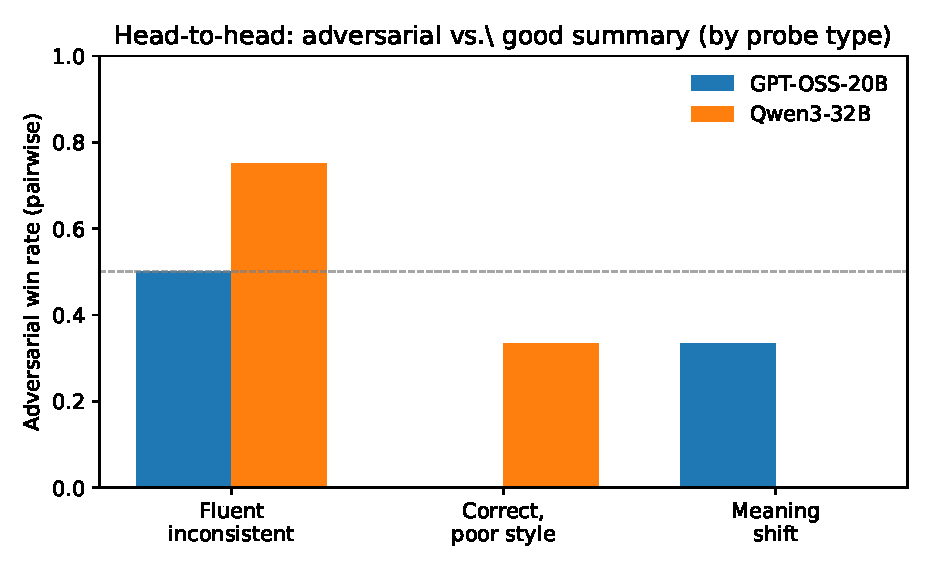
\includegraphics[width=\columnwidth]{adversarial_pairwise_winrate.pdf}
\caption{Pairwise adversarial win rate by probe type (higher means the adversarial summary is preferred over the good one).}
\label{fig:adv}
\end{figure}

\section{Failure Taxonomy}
\label{sec:fail}

We categorize large judge--human discrepancies ($\geq$1.5 points on the Likert scale) into interpretable modes: over-trusting fluency, ignoring factual errors, penalizing correct but awkward text, score inflation/deflation, position-linked reversals, and dimension conflation (near-identical scores across dimensions). Table~\ref{tab:fail} counts how often each mode fires for each judge (tags are not mutually exclusive within the same scored item). Qwen3-32B accumulates far more inflation and ``ignoring factual errors'' events than GPT-OSS-20B, echoing the MAE bias in Table~\ref{tab:mae}. Both judges share the same number of position-linked reversal tags (14), matching the 28\% strict reversal rate in pairwise evaluation. Dimension conflation---assigning nearly identical scores across all four dimensions---occurs on 11\% vs.\ 16\% of tuples (GPT-OSS-20B vs.\ Qwen3-32B), suggesting the latter sometimes collapses the rubric instead of spreading mass across constructs.

\begin{table}[t]
\centering
\footnotesize
\setlength{\tabcolsep}{4pt}
\begin{tabular}{@{}lrr@{}}
\toprule
Failure mode & GPT-OSS-20B & Qwen3-32B \\
\midrule
Ignoring factual errors & 13 & 51 \\
Score inflation & 27 & 149 \\
Score deflation & 12 & 3 \\
Over-trusting fluency & 2 & 14 \\
Position-dependent reversal & 14 & 14 \\
Dimension conflation (count) & 11 & 16 \\
\bottomrule
\end{tabular}
\caption{Rule-based failure tags (non-exclusive counts over scored tuples; see Section~\ref{sec:fail} for definitions).}
\label{tab:fail}
\end{table}

\section{Discussion: Critical Questions}

\paragraph{(1) When do LLM judges align with humans?}
Alignment is strongest when the construct is easy to read off the summary and article together---relevance and coherence for GPT-OSS-20B ($\rho{\approx}0.84$--0.87), with fluency close behind. Consistency remains materially lower for both judges, and Qwen3-32B degrades further on coherence and fluency. Rank metrics are mirrored by calibration: Qwen3-32B inflates coherence--fluency scores by roughly 1.3--1.8 Likert points on average versus humans (Table~\ref{tab:mae}), whereas GPT-OSS-20B's mean absolute errors stay near or below one point on every dimension with smaller signed bias. Rubric mode preserves the same qualitative gap (Table~\ref{tab:rubric}). Pairwise decisions match human majority preference on roughly four out of five decidable articles, but only when order effects do not dominate.

\paragraph{(2) Where do they fail and why?}
Failures concentrate on (i) underestimating subtle inconsistency while surface form stays fluent, as seen in adversarial pairwise rates, (ii) systematic score inflation relative to humans, and (iii) presentation-dependent pairwise reversals. The two judges also disagree most on consistency scores ($\rho{\approx}0.31$ between judges vs.\ ${>}0.56$ on other dimensions), so ``ground truth'' from a single API judge would be unstable precisely where faithfulness matters. Together, these patterns indicate that judges partially substitute fluency and length-invariant heuristics for careful source cross-checking.

\paragraph{(3) Internal consistency.}
Direct, rubric, and pairwise modes are designed to measure the same construct at different granularities; our headline metrics use direct scores for correlation (clean per-dimension signal) and pairwise for order-sensitivity. Direct and rubric scores are nonetheless tightly rank-coupled within each judge ($\rho{\geq}0.80$ on every dimension), so protocol choice mostly shifts absolute levels and human alignment rather than inducing unrelated rankings. Rubric calls still bundle dimensions in one generation step, which can reduce independence across dimensions---consistent with non-trivial conflation rates (Table~\ref{tab:fail}).

\paragraph{(4) Prompt sensitivity.}
Consistency correlation moves by several hundredths of a point across minimal, standard, and cot variants (std.\ ${\sim}0.04$--0.06), larger than for relevance. Reference inclusion helps consistency alignment slightly, supporting the use of reference text when faithfulness is paramount.

\paragraph{(5) Can LLM judges replace human evaluation?}
Not as a sole gatekeeper for research-quality summarization evaluation: while aggregate $\rho$ is encouraging on several dimensions, order effects, inflation, and adversarial slip on fluent-but-wrong text show that human oversight remains necessary, especially for consistency. GPT-OSS-20B is closer to humans on average in this study, but both models exhibit failure modes that a correlation summary alone would hide.

\section{Conclusion}

We hypothesized dimension-specific judge weakness and found it: consistency with the source trails other SummEval dimensions under Spearman correlation for two modern API judges, with Qwen3-32B showing a larger gap and more inflation-style errors. Mean-absolute-error and failure-tag analyses corroborate systematic leniency for Qwen3-32B and tighter calibration for GPT-OSS-20B, while inter-judge agreement is weakest exactly on consistency ($\rho{\approx}0.31$). Pairwise agreement with humans is moderate-to-good on aggregate yet undermined by order sensitivity; adversarial probes further show that fluent inaccuracies can win head-to-head. These results support using LLM judges as \emph{assistive} tools with explicit bias checks, not drop-in replacements for human rubrics.

\section*{Limitations}

The study uses 50 English news articles and two small summarizers; findings may not transfer to long-form, multilingual, or frontier-model outputs. Student annotators are not professional editors. Hosted models and rate limits change over time; numerical results are tied to the reported API versions.

\section*{Ethics Statement}

Annotators were informed of workload; article text and model outputs are used only for coursework. API providers process prompts under their terms; we do not deploy judges for end-user decisions.

\section*{Acknowledgements}

This report was prepared for the course \textit{Evaluation Methods in NLP} (2026).

\bibliography{custom}
\bibliographystyle{acl_natbib}

\appendix

\section{Annotation and judge prompts (abridged)}

\paragraph{Human dimensions.}
Annotators see short definitions mirroring SummEval: coherence emphasizes global structure; consistency requires that all supporting facts appear in the article; fluency covers grammar and readability; relevance covers salient content without padding.

\paragraph{Direct scoring (standard variant, sketch).}
The judge receives the article, the summary, optional reference highlights, and a rubric paragraph for the target dimension, then outputs a single integer 1--5. The \emph{minimal} variant shortens instructions; the \emph{cot} variant asks for step-by-step reasoning before the score.

\paragraph{Pairwise (standard variant, sketch).}
The judge compares two summaries ``overall'' with respect to coherence, consistency, fluency, and relevance, and replies with a single letter indicating which summary is better.

\paragraph{Rubric (standard variant, sketch).}
The judge receives all four dimension definitions at once and returns four integers in a fixed key--value format.

\section{Reproducibility}

The study subset, model outputs, annotations, aggregated gold, judge logs, and numerical analysis summaries are versioned together in the course repository.

\end{document}
